\scanpage{9}
\mspage{3}

B) Courbes \inserted{ell.} anharmoniques de type hexagonal.

La catégorie de ces courbes équivalente \unsure{:|;|à} celle des hexagones orientés, i.e. des torseurs $S$ sous
\[
\begin{aligned}
\mathbb Z/6\mathbb Z&\simeq\mu_6(\mathbb C)\simeq
\text{groupe des}\\
&\qquad\text{unités \inserted{alg.} de }Q(\underset{\zeta}{\underline{\sqrt[3]{1}}})\\
&\simeq\text{groupe des unites \unsure{de}}\\
&\qquad\text{\uline{de}}\ \deleted{\mathbb Z[\zeta]=\mathbb Z(T]/}\\
&\qquad\mathbb Z[\zeta]=\mathbb Z[T]/(1+T+T^2)\\
&\qquad(\zeta=\exp 2i\pi/3)
\end{aligned}
\]

\figure{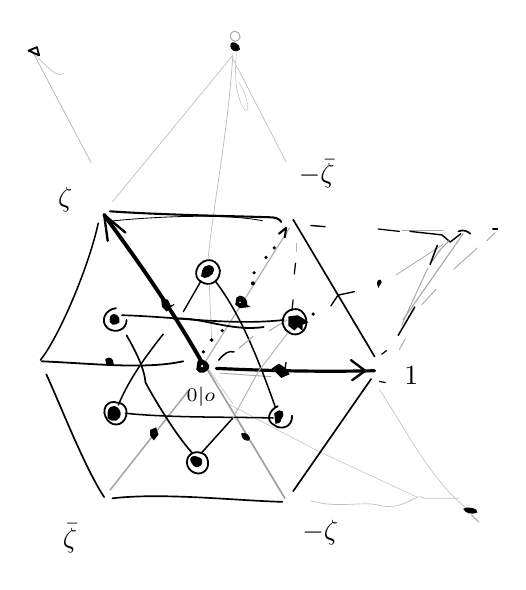
\begin{tikzpicture}[x=.015cm,y=-.015cm,line cap=round,line join=round]
\draw[gray!60,line width=.25pt] (171,917)--(221,1012);
\draw[gray!50,line width=.25pt] (174,921).. controls (183,930) and (193,941) .. (197,936);
\draw[gray!50,line width=.25pt] (239,1045)--(340,922)--(386,1011);
\draw[gray!55,line width=.25pt] (341,920).. controls (337,985) and (324,1050) .. (320,1093);
\draw[gray!45,line width=.22pt] (344,919).. controls (341,947) and (347,962) .. (351,967)
 .. controls (357,971) and (352,952) .. (346,944);
\draw[gray!50,line width=.25pt] (321,1114)--(323,1162);
\draw[gray!45,line width=.25pt] (320,1186)--(341,1216);
\draw[gray!45,line width=.22pt] (337,1216)--(413,1256)--(497,1295);
\draw[gray!45,line width=.25pt] (465,1204).. controls (487,1236) and (507,1280) .. (542,1307);
\draw[gray!50,line width=.25pt] (407,1298).. controls (429,1305) and (452,1298) .. (465,1302)
 .. controls (487,1307) and (496,1290) .. (503,1296)--(532,1296);
\draw[line width=.55pt] (227,1063).. controls (219,1100) and (194,1159) .. (178,1179);
\draw[line width=.6pt] (183,1191).. controls (195,1217) and (215,1269) .. (232,1295);
\draw[line width=.6pt] (239,1296).. controls (282,1291) and (344,1298) .. (383,1299);
\draw[line width=.6pt] (392,1290)--(458,1195);
\draw[line width=.6pt] (461,1176)--(392,1060);
\draw[line width=.75pt] (237,1053).. controls (280,1056) and (339,1057) .. (371,1058)
 .. controls (377,1058) and (380,1059) .. (382,1062);
\draw[line width=.3pt] (240,1061).. controls (282,1057) and (336,1055) .. (366,1061);
\draw[line width=.65pt] (179,1180).. controls (225,1182) and (266,1187) .. (299,1180);
\draw[gray!70,line width=.55pt] (237,1289)--(304,1204);
\draw[gray!60,line width=.45pt] (316,1183)--(389,1067);
\draw[gray!75,line width=.6pt] (320,1188)--(385,1296);
\draw[line width=1.4pt] (316,1183).. controls (286,1130) and (258,1092) .. (232,1056);
\draw[line width=.85pt] (235,1078)--(232,1056)--(250,1071);
\draw[line width=1.15pt] (327,1186).. controls (371,1188) and (413,1189) .. (461,1188);
\draw[line width=.85pt] (441,1179)--(453,1188)--(442,1196);
\draw[gray!65,line width=.35pt] (330,1190)--(373,1193);
\draw[line width=.75pt] (380,1072)--(386,1067)--(385,1075);
\draw[line width=.5pt] (314,1112)--(299,1138);
\draw[line width=.55pt] (282,1157).. controls (263,1181) and (252,1198) .. (244,1217);
\draw[line width=.55pt] (326,1112).. controls (345,1137) and (359,1168) .. (377,1219);
\draw[line width=.55pt] (250,1224).. controls (288,1228) and (341,1227) .. (375,1228);
\draw[line width=.6pt] (247,1141).. controls (290,1142) and (340,1150) .. (384,1145);
\draw[line width=.65pt] (291,1144).. controls (314,1142) and (338,1155) .. (367,1151);
\draw[line width=.6pt] (251,1158).. controls (259,1172) and (266,1186) .. (267,1198)
 .. controls (274,1211) and (291,1240) .. (306,1257);
\draw[line width=.55pt] (314,1258)--(341,1228);
\draw[gray!60,line width=.35pt] (341,1228)--(363,1188)--(389,1154);
\draw[line width=.55pt] (329,1179).. controls (334,1173) and (337,1171) .. (342,1172);
\draw[gray!65,line width=.4pt] (346,1169)--(358,1159);
\draw[gray!65,line width=.4pt] (372,1154)--(387,1145);
\draw[line width=.45pt] (391,1137)--(392,1128);
\draw[line width=.45pt] (393,1106)--(394,1097);
\draw[gray!55,line width=.3pt] (395,1080)--(395,1087);
\draw[line width=.5pt] (424,1133)--(430,1124)--(444,1121);
\draw[gray!65,line width=.3pt] (479,1107)--(519,1081);
\draw[line width=.45pt] (464,1068)--(482,1070);
\draw[gray!70,line width=.3pt] (484,1069)--(519,1069);
\draw[line width=.5pt] (491,1070)--(518,1073)--(525,1079)--(534,1072);
\draw[gray!75,line width=.4pt] (524,1078)--(517,1085)--(510,1095);
\draw[line width=.55pt] (508,1098)--(514,1082);
\draw[gray!70,line width=.35pt] (484,1149)--(506,1101);
\draw[line width=.55pt] (481,1158)--(495,1134);
\draw[gray!70,line width=.4pt] (485,1145)--(536,1072);
\draw[line width=.6pt] (532,1070).. controls (536,1068) and (540,1070) .. (542,1072);
\draw[gray!65,line width=.35pt] (482,1170)--(487,1161);
\draw[gray!65,line width=.35pt] (501,1132)--(513,1119);
\draw[gray!65,line width=.35pt] (528,1102)--(548,1084);
\draw[gray!65,line width=.35pt] (556,1078)--(563,1071);
\draw[line width=.45pt] (561,1068)--(565,1068);
\draw[line width=.5pt] (407,1065)--(419,1066);
\draw[line width=.45pt] (467,1174)--(471,1171);
\draw[line width=.45pt] (465,1197)--(470,1198);
\draw[line width=.65pt] (168,917)--(175,914)--(177,921)--cycle;
\draw[gray!65,line width=.4pt] (339,906).. controls (338,898) and (347,899) .. (347,906)
 .. controls (345,910) and (341,910) .. (339,906);
\fill (339,911).. controls (341,908) and (347,911) .. (347,916)
 .. controls (344,919) and (338,918) .. (339,911);
\fill (536,1305).. controls (540,1302) and (549,1305) .. (548,1308)
 .. controls (543,1310) and (538,1309) .. (536,1305);
\draw[gray!65,line width=.4pt] (543,1310)--(549,1316);
\draw[line width=.65pt] (330,1103).. controls (330,1111) and (324,1116) .. (317,1114)
 .. controls (307,1111) and (309,1101) .. (314,1097)
 .. controls (320,1092) and (328,1094) .. (330,1103);
\fill (315,1103).. controls (317,1097) and (325,1097) .. (325,1103)
 .. controls (325,1107) and (317,1112) .. (314,1108)--cycle;
\draw[line width=.65pt] (251,1145).. controls (251,1153) and (242,1157) .. (235,1152)
 .. controls (228,1146) and (233,1136) .. (242,1135);
\fill (237,1142).. controls (241,1137) and (246,1142) .. (245,1147)
 .. controls (242,1150) and (235,1151) .. (237,1142);
\draw[line width=.65pt] (403,1144).. controls (405,1154) and (396,1160) .. (389,1156)
 .. controls (379,1150) and (383,1137) .. (392,1136)
 .. controls (398,1135) and (401,1138) .. (403,1144);
\fill (388,1142)--(396,1141)--(401,1144)--(405,1147)--(400,1149)
 --(400,1154)--(396,1151)--(393,1154)--(388,1150)--cycle;
\draw[line width=.65pt] (251,1223).. controls (251,1233) and (241,1237) .. (235,1230)
 .. controls (228,1221) and (235,1212) .. (243,1215)
 .. controls (248,1215) and (251,1219) .. (251,1223);
\fill (235,1223).. controls (236,1215) and (245,1217) .. (246,1224)
 .. controls (246,1230) and (240,1233) .. (235,1228)--cycle;
\draw[line width=.65pt] (391,1226).. controls (392,1235) and (382,1239) .. (376,1234)
 .. controls (368,1230) and (372,1221) .. (379,1218);
\fill (376,1224).. controls (383,1218) and (386,1224) .. (382,1229)
 .. controls (382,1232) and (379,1233) .. (377,1233)--cycle;
\draw[line width=.65pt] (320,1265).. controls (321,1273) and (313,1278) .. (306,1273)
 .. controls (299,1268) and (302,1257) .. (310,1257)
 .. controls (317,1257) and (319,1260) .. (320,1265);
\fill (305,1264).. controls (304,1258) and (314,1260) .. (315,1264)
 .. controls (316,1270) and (308,1273) .. (305,1264);
\fill (233,1178).. controls (237,1175) and (240,1178) .. (240,1182)
 .. controls (238,1185) and (233,1185) .. (233,1178);
\fill (280,1126)--(286,1128)--(289,1134)--(285,1138)--(281,1134)--cycle;
\draw[line width=.45pt] (286,1135)--(291,1132);
\fill (344,1126).. controls (347,1122) and (354,1126) .. (353,1132)
 --(356,1134)--(347,1135)--(343,1132)--cycle;
\fill[white] (347,1130) circle[radius=.35pt];
\fill (374,1186)--(380,1182)--(386,1186)--(389,1191)--(382,1194)--cycle;
\draw[line width=.5pt] (385,1187)--(386,1181);
\fill (271,1238)--(276,1236)--(278,1242)--(274,1247)--(271,1243)--cycle;
\fill (348,1241).. controls (352,1239) and (357,1244) .. (355,1247)
 .. controls (352,1248) and (348,1246) .. (348,1241);
\fill (311,1180).. controls (312,1177) and (319,1178) .. (321,1184)
 .. controls (321,1190) and (312,1192) .. (310,1187)--cycle;
\fill[white] (315,1184) circle[radius=.45pt];
\fill (316,1172) circle[radius=.65pt];
\fill (323,1162) circle[radius=.7pt];
\fill (332,1154) circle[radius=.65pt];
\fill (358,1114) circle[radius=.75pt];
\fill (359,1105) circle[radius=.65pt];
\fill (369,1092) circle[radius=.65pt];
\fill (376,1084) circle[radius=.65pt];
\fill (409,1140) circle[radius=.65pt];
\fill (463,1114).. controls (463,1110) and (467,1110) .. (467,1113)
 --(464,1118)--cycle;
\node at (199,1043) {$\zeta$};
\node at (412,1021) {$-\bar\zeta$};
\node at (492,1192) {$1$};
\node at (203,1330) {$\bar\zeta$};
\node at (415,1325) {$-\zeta$};
\node[font=\scriptsize] at (314,1210) {$\unsure{0|o}$};
\end{tikzpicture}}

\deleted{\unsure{On pourra|On pose}} \inserted{On pose}
\[
\mathbb E\ell_1\unsure{\deleted{(S))}|\deleted{(S)}}\simeq\mathbb C/\mathbb Z[\zeta]
\]
\[
\mathbb E\ell_1(S)\simeq\mathbb E\ell_1\mathbin{\wedge}_{\mathbb Z/6\mathbb Z}S
\]

\uline{Construction} On réalise l'hexagone comb. $S$ euclidiennement (canonique), dans \unsure{vectoriel} euclidien $V_S$, \deleted{\unsure{centre}} \inserted{origine} etant le barycentre de $S$. On désigne par $V_S$ le \deleted{\unsure{lattice}} \inserted{réseau} engendré par $S$, et
\[
X_S=\mathbb E\ell_1(S)\simeq V_S/\Gamma_S
\]
La structure euclidienne \uline{orientée} de $V_S$ definit la structure complexe de $X_S$.

\margin{8}
